%----------------------------------------------------------------------------------------
%	Section: PRo3D Command Line Interface
%----------------------------------------------------------------------------------------
\section{Surface Comparison Extension}

PRo3D can be used to compare features of two surfaces. To activate the surface comparison features, go to the menu and select \emph{Change Mode} and then \emph{Surface Comparison}. You will see the Surface Comparison features (figure  \ref{fig:surfaceComparison}).


\begin{figure}[h]
	\centering
	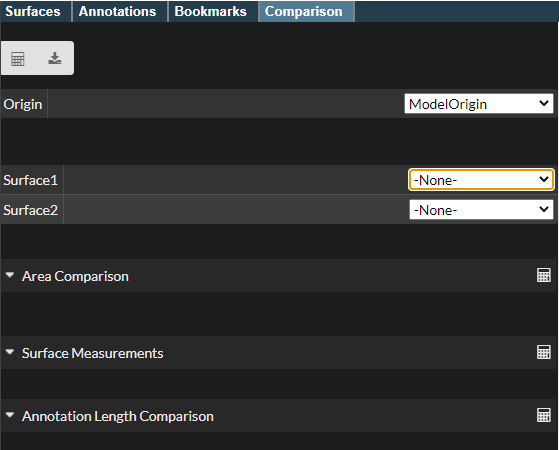
\includegraphics[width=0.6\textwidth]{pics/surfaceComparison.PNG}
	\caption[The surface comparison interface.]{The Surface Comparison Interface.}
	\label{fig:surfaceComparison}
\end{figure}

Use the drop down labelled \emph{Origin} to select which point should be used as the centre of a surface for various calculations.

In the drop down boxes labelled \emph{Surface1} and \emph{Surface2} you can select the surfaces you wish to compare. Once you have selected two surfaces, you can toggle their visibility using the \texttt{t} button on your keyboard. The calculation of surface measurements is also triggered by selecting two surfaces. You can update the measurements by clicking on the button with the calculator icon. To export all measurements click on button with the download icon. The measurements will be saved in the PRo3D home directory. The full path is printed on the console when exporting.

\subsection{Comparing Selected Areas}

Make sure that two surfaces are loaded and selected in the \emph{Comparison} tab. In the menu bar above the 3D-View, choose \emph{Select Area} from the drop down (figure \ref{fig:surfaceComparisonAreaSelection}).

\begin{figure}[h]
	\centering
	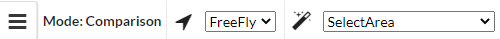
\includegraphics[width=0.8\textwidth]{pics/surfaceComparisonSelectArea.PNG}
	\caption[Selecting an area to compare.]{Selecting an area to compare.}
	\label{fig:surfaceComparisonAreaSelection}
\end{figure}

Hold the control key on your keyboard and click on a point on a surface to choose a location. You might need to click twice, if the 3D-View is not in focus. Once you have selected a location, a translucent sphere indicates the selected area (figure \ref{fig:surfaceComparisonAreaSphere}). You can make this sphere smaller by pressing the \emph{minus} key, bigger by pressing the \emph{plus} key on your keyboard. All vertices within a certain distances to the selected location are taken into account (in other words, the area is spherical).

\begin{figure}[h]
	\centering
	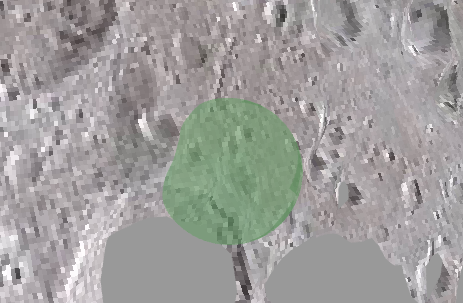
\includegraphics[width=0.6\textwidth]{pics/surfaceComparisonAreaSphere.PNG}
	\caption[A selected area.]{A selected area.}
	\label{fig:surfaceComparisonAreaSphere}
\end{figure}

All areas you have created are displayed in a list (figure \ref{fig:surfaceComparisonAreaList}). If you wish to change the location of an area, simply delete it by clicking on the red cross and select a new location. 

\begin{figure}[h]
	\centering
	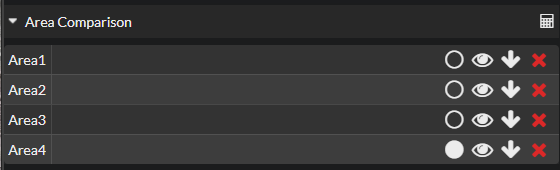
\includegraphics[width=0.6\textwidth]{pics/surfaceComparisonAreaList.PNG}
	\caption[Selecting an area to compare.]{Selecting an area to compare.}
	\label{fig:surfaceComparisonAreaList}
\end{figure}

In figure \ref{fig:surfaceComparisonAreaList}, \emph{Area4} is selected. With the eye icon button you can set the visibility of an area. The arrow icon can be used to toggle the resolution of the vertex statistics analysis between lower and higher. This has a big effect if the two surfaces have a very different resolutions, and determines the vertices of which surface are used as a basis to calculate and visualise the differences between the two surfaces.

Once an area is to your liking, update the measurements by clicking on the calculator icon or button. Depending on the size of the area and the resolution of the surfaces, this might take a few seconds.

\begin{figure}[h]
	\centering
	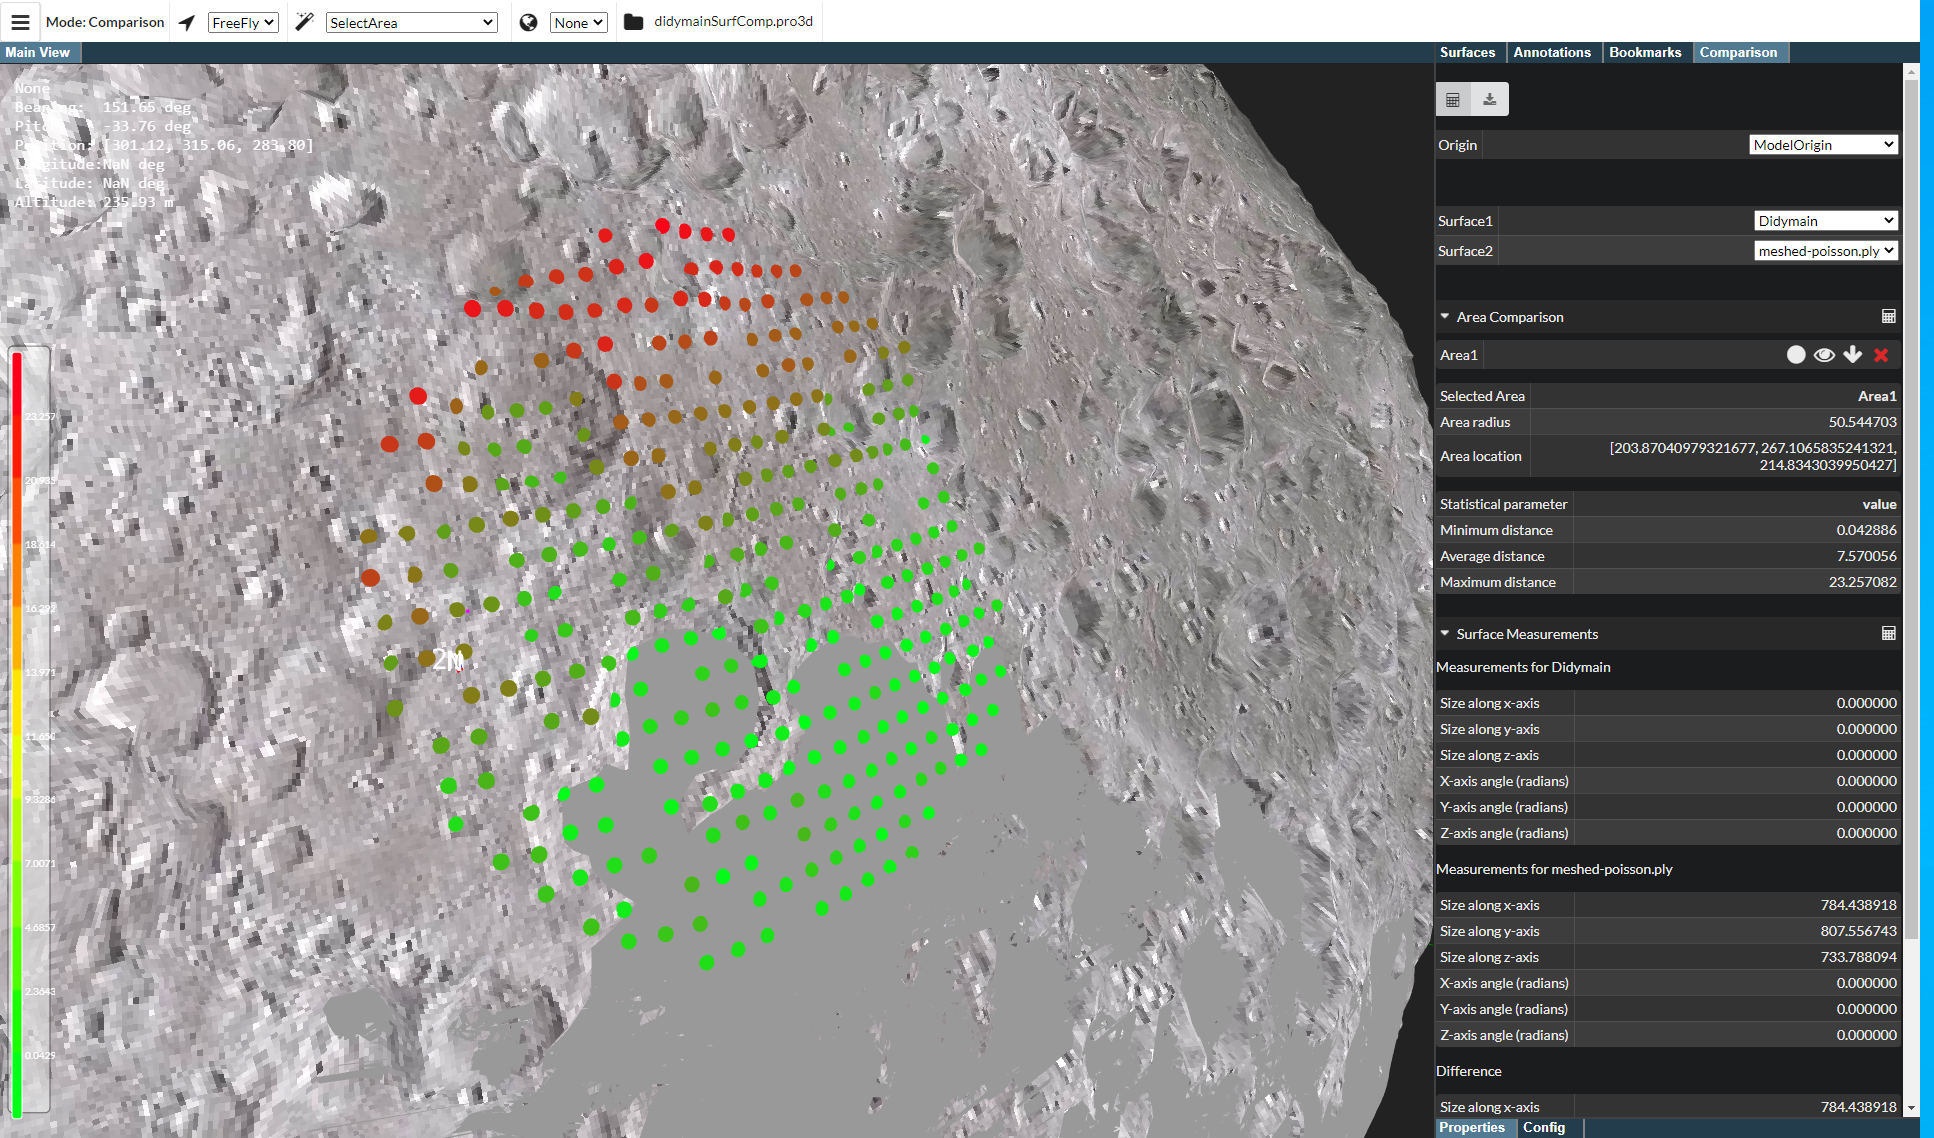
\includegraphics[width=1.0\textwidth]{pics/surfaceComparisonArea3DView1.PNG}
	\caption[Comparing an area of two surfaces.]{Comparing an area of two surfaces.}
	\label{surfaceComparisonArea3DView1.PNG}
\end{figure}

Each location that was used to calculate the distance between the two surfaces is visualised with a coloured sphere (figure \ref{surfaceComparisonArea3DView1.PNG}). The colour of the sphere encodes the distance, with red encoding large distances and green small distances. The concrete values assigned to each colour can be seen on the legend on the left. Area size, area location, and statistic parameters are displayed on the right hand side for the selected area. The legend is always valid for the selected area.

\begin{figure}[h]
	\centering
	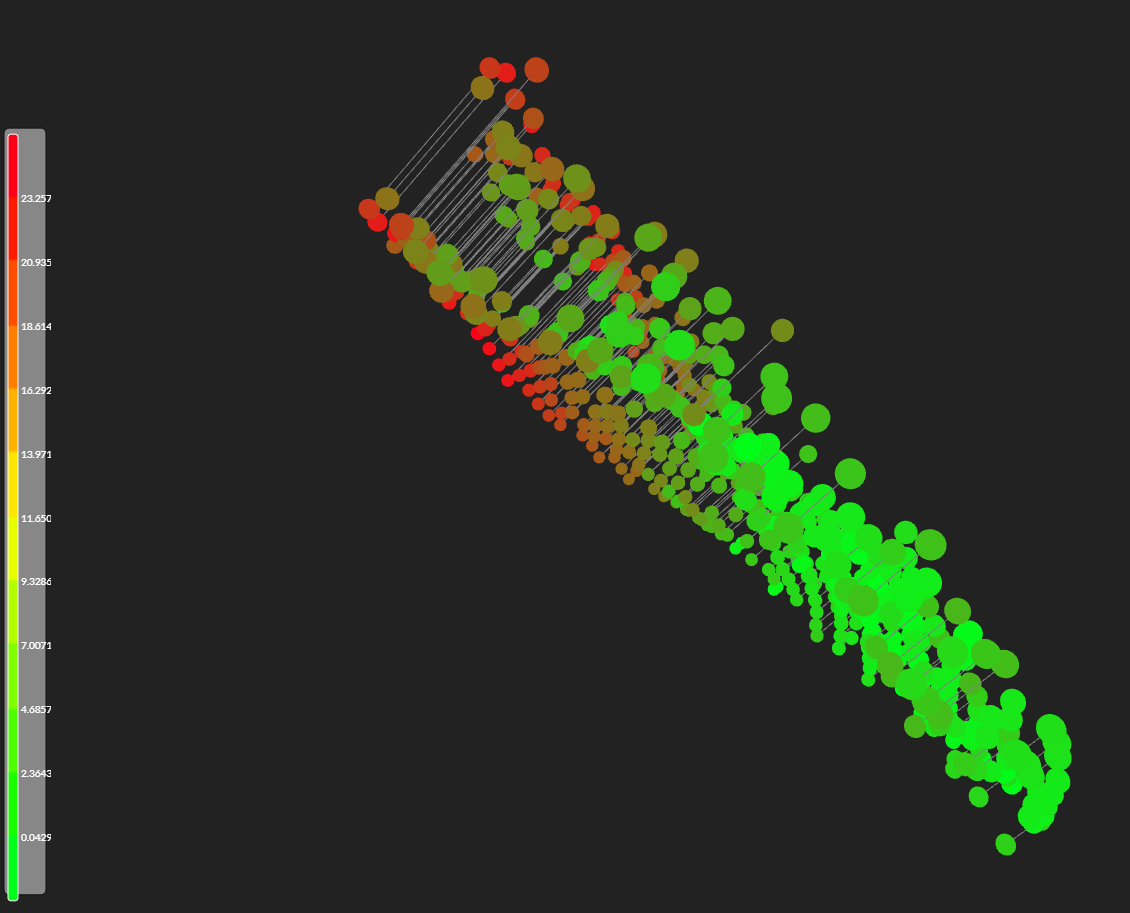
\includegraphics[width=0.8\textwidth]{pics/surfaceComparisonArea3DView2.PNG}
	\caption[Visualising the differences between two surfaces.]{Visualising the differences between two surfaces on a vertex level. The surfaces have been set to invisible.}
	\label{surfaceComparisonArea3DView2.PNG}
\end{figure}

To explore the differences between the two surfaces in more detail, set one or both areas to invisible (in the surfaces tab, use the eye icon). Figure \ref{surfaceComparisonArea3DView2.PNG} shows the difference visualisation with both areas set to invisible.

\clearpage
\subsection{Comparing Length Measurements}

To compare length measurements, create a bookmark and make sure it is selected. This bookmark can now be used as a projection point for annotations. For this, select the Bookmark projection mode for annotation drawing (figure \ref{fig:surfaceComparisonBookmarkMode}).

\begin{figure}[h]
	\centering
	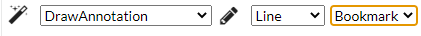
\includegraphics[width=0.7\textwidth]{pics/surfaceComparisonBookmarkMode.PNG}
	\caption[The Bookmark Projection Mode.]{The Bookmark projection mode for comparing length measurements on two surfaces. Make sure a bookmark is selected when using this mode.}
	\label{fig:surfaceComparisonBookmarkMode}
\end{figure}

Now draw one annotation on each of the two surfaces while the same bookmark is selected. Use the \texttt{t} button on your keyboard to toggle visibility between the two surfaces. Return to the comparison window and click the button with the calculator icon to update the calculations. The measurements for annotations are listed under the heading \emph{Annotation Length Comparison}.

Bookmarks can be exported and imported using the menu. Select the main menu (top left), then \emph{Bookmarks}, then \emph{Import} or \emph{Export}.